\documentclass[border=5pt]{standalone}
\usepackage{tikz}
\usepackage{amsmath,amssymb}
\usetikzlibrary{shapes.geometric, arrows.meta, positioning}

\definecolor{purplebox}{HTML}{EEEDFE}
\definecolor{purpleborder}{HTML}{534AB7}
\definecolor{purpletext}{HTML}{3C3489}
\definecolor{bluebox}{HTML}{E6F1FB}
\definecolor{blueborder}{HTML}{185FA5}
\definecolor{bluetext}{HTML}{0C447C}
\definecolor{greenbox}{HTML}{E1F5EE}
\definecolor{greenborder}{HTML}{0F6E56}
\definecolor{greentext}{HTML}{085041}
\definecolor{bluelight}{HTML}{F8FBFE}
\definecolor{bluelightborder}{HTML}{85B7EB}
\definecolor{greenlight}{HTML}{F2FBF7}
\definecolor{greenlightborder}{HTML}{5DCAA5}
\definecolor{grayline}{HTML}{D3D1C7}
\definecolor{graytext}{HTML}{5F5E5A}

\begin{document}
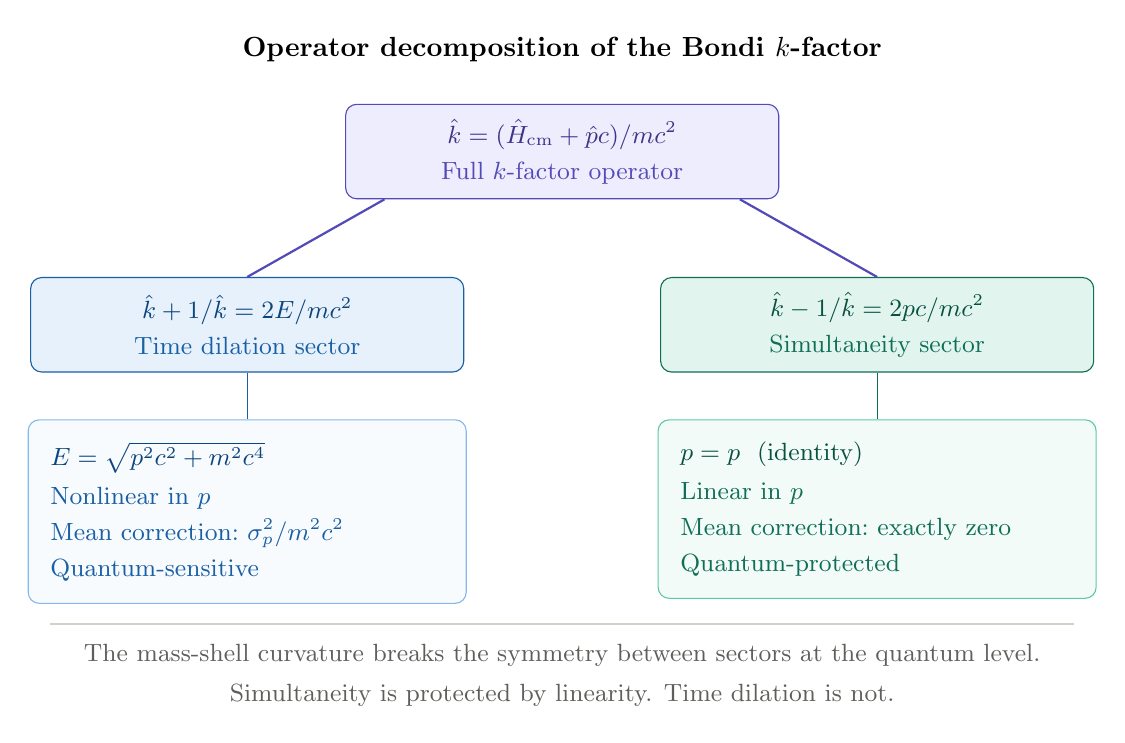
\begin{tikzpicture}[
    mainbox/.style={rectangle, rounded corners=4pt, minimum width=5.5cm, minimum height=1.2cm, align=center},
    detailbox/.style={rectangle, rounded corners=4pt, minimum width=5.5cm, minimum height=2.2cm, align=left, text width=5cm, inner sep=8pt},
    every node/.style={font=\small}
]

% Title
\node[font=\bfseries] at (0, 5.5) {Operator decomposition of the Bondi $k$-factor};

% Top box
\node[mainbox, fill=purplebox, draw=purpleborder] (top) at (0, 4.2)
    {\textcolor{purpletext}{\bfseries $\hat{k} = (\hat{H}_{\mathrm{cm}} + \hat{p}c) / mc^2$} \\[2pt]
     \textcolor{purpleborder}{\small Full $k$-factor operator}};

% Left branch
\node[mainbox, fill=bluebox, draw=blueborder] (left) at (-4, 2)
    {\textcolor{bluetext}{\bfseries $\hat{k} + 1/\hat{k} = 2E / mc^2$} \\[2pt]
     \textcolor{blueborder}{\small Time dilation sector}};

% Right branch
\node[mainbox, fill=greenbox, draw=greenborder] (right) at (4, 2)
    {\textcolor{greentext}{\bfseries $\hat{k} - 1/\hat{k} = 2pc / mc^2$} \\[2pt]
     \textcolor{greenborder}{\small Simultaneity sector}};

% Connecting lines
\draw[purpleborder, thick] (top.south west) ++(.5,0) -- (left.north);
\draw[purpleborder, thick] (top.south east) ++(-.5,0) -- (right.north);

% Left detail
\node[detailbox, fill=bluelight, draw=bluelightborder, anchor=north] (leftdet) at (-4, 0.8)
    {\textcolor{bluetext}{$E = \sqrt{p^2c^2 + m^2c^4}$} \\[3pt]
     \textcolor{blueborder}{\small Nonlinear in $p$} \\[2pt]
     \textcolor{blueborder}{\small Mean correction:\ $\sigma_p^2 / m^2c^2$} \\[2pt]
     \textcolor{blueborder}{\small Quantum-sensitive}};

% Right detail
\node[detailbox, fill=greenlight, draw=greenlightborder, anchor=north] (rightdet) at (4, 0.8)
    {\textcolor{greentext}{$p = p$\ \ (identity)} \\[3pt]
     \textcolor{greenborder}{\small Linear in $p$} \\[2pt]
     \textcolor{greenborder}{\small Mean correction:\ exactly zero} \\[2pt]
     \textcolor{greenborder}{\small Quantum-protected}};

% Connecting lines to detail
\draw[blueborder] (left.south) -- (leftdet.north);
\draw[greenborder] (right.south) -- (rightdet.north);

% Bottom line and text
\draw[grayline] (-6.5, -1.8) -- (6.5, -1.8);
\node[font=\small, text=graytext] at (0, -2.2) {The mass-shell curvature breaks the symmetry between sectors at the quantum level.};
\node[font=\small, text=graytext] at (0, -2.7) {Simultaneity is protected by linearity. Time dilation is not.};

\end{tikzpicture}
\end{document}
